\subsection{Purpose}
This paper represents the \textbf{R}equirement \textbf{A}nalysis and \textbf{S}pecification \textbf{D}ocument of the \textit{System Under Development}, which will implement the \emph{PowerEnJoy Car-Sharing} Service. This document aims at explaining the functionalities of the System in terms of Functional Requirements, NonFunctional Requirements and Special Requirements, represented using both diagrams and natural language.

%\newcounter{GoalCounter}
%\stepcounter{GoalCounter}

The above is a comprehensive list of functionalities provided by the System, that actually translates to a list of goals that the system should reach.

\begin{enumerate}
	\item[G1] The System should allow the registration of the Visitors with their credentials and payment informations.
	\item[G2] The System should allow all Users to use all the functionalities reserved to them.
	\item[G3] The System should be able to give each User the list of all the available cars in a range of 5KM from his/her GPS position or a specific address.
	\item[G4] The System should allow each of its Users to reserve a Car whose state is Available.
	\item[G5] If an User has reserved a Car and he/she did not unlock it within 1 hour from the reservation, the System sets the Car state as Available, the reservation expires and the user pays a fixed Fee of 1 EUR.  
	\item[G6] The system should allow each User to unlock a previously reserved Car when he/she is in a distance range of 15 meters from the same Car.
	\item[G7] The system should allow each User to drive a Car which he/she has previously unlocked.
	\item[G8] The System should be able to know the time usage of the Car, misured in minutes.
	\item[G9] The System should allow Users to know where are the Parking Areas.
	\item[G10] The system should allow each User to end the ride in a Parking Area.
	\item[G11] If the System detects the User took at least two other passengers onto the Car, the system applies a discount of 10\% on the last ride. 
	\item[G12] If a Car is left with no more than 50\% of the battery empty, the System applies a discount of 20\% on the last ride. 
	\item[G13] If a Car is left at special parking areas where they can be recharged and the User takes care of plugging the Car into the power grid, the System applies a discount of 30\% on the last ride. 
	\item[G14] If a Car is left at more than 3 KM from the nearest Charging Area or with more than 80\% of the battery empty, the system charges 30\% more on the last ride to compensate for the cost required to recharge the car on-site.
	\item[G15] If the User enables the money saving option, he/she can input his/her final destination and the System provides the address of the Charging Area where to leave the Car in order to get a Discount on the total Fee. The Charging Area is determined by the System to ensure a uniform distribution of Cars in the city and depends both on the destination of the User and on the availability of Sockets at the selected Charging Area. 
\end{enumerate}


\subsection{Intended Audience}
This document is addressed to all the stakeholders involved in the \emph{PowerEnJoy} project. This includes, but it is not limited to, the development committee, product designers and engineers, quality assurance, who will decide if the requirements described in this document have met the intended system requirements.

%TODO Migliorare
\subsection{Product Scope}
%TODO Add The World and the Machine here
The aim of the \emph{PowerEnJoy} project is to provide a \textit{Car-Sharing} Service which implements electric-powered cars only.
This system will have to interface the Cars, Charging Areas, allowing Users to reserve, unlock, drive and park Cars, finally charging them the cost of the ride. 
The System will keep track of Cars' position, battery level, possible damages, plugging state.

%TODO Add sth here
\begin{figure}[!htbp]
\centering
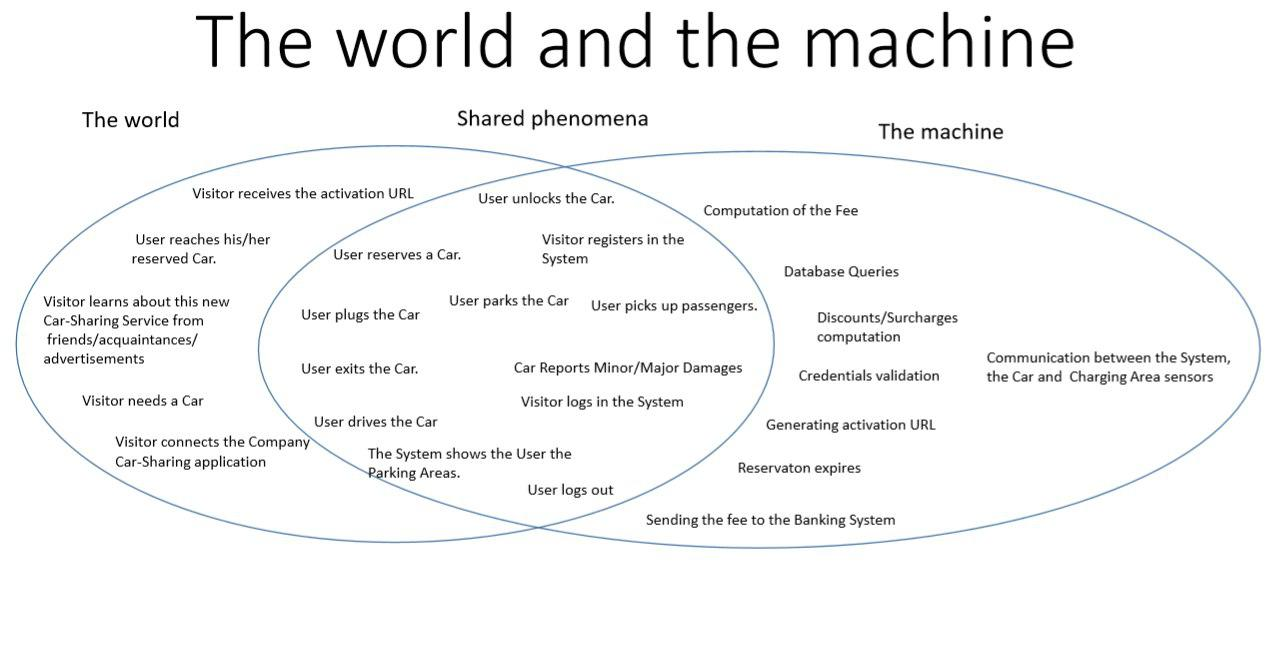
\includegraphics[width=\linewidth,keepaspectratio]{../The_world_and_the_machine.jpg}
\caption{The World And The Machine}
\end{figure}
\FloatBarrier

\subsection{Definitions, Acronyms and Abbreviations}
\subsubsection{Business terms glossary}
\begin{itemize}
	\item \emph{Account} \\
	An Account is a virtual representation of a User in the System. The System can read and store information about a User.
	
	\item \emph{Application} \\
	It's the software interface between the User and the System, which allows the User to access the System functionalities.
	
	\item \emph{Battery} \\
	A Battery powers a Vehicle. The charge state of the Battery can be anywhere between 0\% and 100\%, is reduced when the Vehicle is In Use, and increases when the Vehicle is Plugged to a Charging Area.

	
	\item \emph{Car} \\
	An electric car owned by the Car-sharing service, rented to the User and tracked by the System.The Car communicates to the System its position, the status of its battery, its damages, the connection to an electrical socket and the number of seats occupied. A Car has a status and a Plugged flag, the status can be:
	\begin{itemize}
		\item \textit{In Use}, if the engine is turned on. In this state, it cannot be Reserved by an User.
		\item \textit{Available}, if it can be Reserved by an User.
		\item \textit{Reserved}, if an User has reserved it but has still not unlocked it.
		\item \textit{Unavailable} if it can't be \textit{Reserved} by any User (for example due to damage, battery exhaustion, mainteinance, ...)
	\end{itemize}
	Additionally, the \textit{Plugged} flag indicates if the {Car} is plugged or not to the socket of the Charging Area.
	
	\item \emph{Car-sharing} \\
	A Car-sharing service allows Users to rent Cars for a limited amount of time, being charged a Fee according to time and possibly applying a Discount or an Increase.
	
	\item \emph{Charging Area} \\		
	A special Parking Area where Cars plugs can be connected to the socket in order to recharge their Battery.	

	\item \emph{Company} \\
	The enterprise that wants to build the System to provide a \textit{Car-Sharing} Service. It represents the main stakeholder.	
	
	\item \emph{Database} \\
	A structure that holds all the information used by the System. For instance, a Database could hold records of every User, Car, every time a User rented a Car,and so on.

	\item \emph{Discount} \\
	A reduction in the Fee because of good behaviour on the part of the User, e.g. leaving the Cars plugged or bringing it back with a mostly-full battery. The actions that constitute good behaviour are determined ad detailed further in the document.

	\item \emph{Employee}\\
	He's an employee of the Company which is charged of every kind of maintenance of the Car (Charging the Car battery on-site, moving a Car to a Charging Area and so on). The employees are handled by an External System

	\item \emph{Fee}\\
	The amount of money that the User will be charged for their usage of the Car-sharing service, or for making a Reservation that is not fulfilled.

	\item \emph{GPS}\\
	Global Positioning System, it's widely used in our System.

	\item \emph{Surcharge}\\
	An increase in the Fee caused by an improper behaviour on the part of the User, e.g. bringing the Cars back with a mostly-empty battery.

	\item \emph{Parking Area}\\
	A place where the User can leave their Car and exit it to end the Ride. Parking Areas are predefined by the System.

	\item \emph{Passenger}\\
	A person, different from the User, who travels in a Car together with an User. 

	\item \emph{Plug}\\
	A part of the Car that can be inserted in a Socket of a Charging Area.

	\item \emph{Ride}\\
	Represents the travel done with the Car by the User. It starts from the moment the User ignites the engine of the Car and ends when the Car is parked in a Parking Area,the User and all the other passengers exit the Car.

	\item \emph{Reservation}\\
	A User performs a Reservation in order to book an Available Car for a maximum of 1 hour. In this time period the Car is assigned to the specific User only. An User can only have one active Reservation at time.

	\item \emph{Socket}\\
	A part of the Charging Area that can be connected with the Plug of a Car. 

	\item \emph{System}\\
	The software structure this document is about.

	\item \emph{User}\\
	A person registered on the System, who has access to the Car-Sharing Service functionalities.

	\item \emph{Visitor}\\
	A person who needs to log in the System to access the Car-Sharing Service functionalities.
\end{itemize}

\subsubsection{External systems}
\begin{itemize}
	\item \emph{Banking System}
	An external system that allows the System to charge the users for a Fee.
	
	\item \emph{Mail System}
	An external system that allows to send emails to Visitors and Users.

	\item \emph{Mapping System}
	An external system that is designed to capture, store, manipulate, analyze, manage, and present spatial or geographical data. 
	It is used in particular to show the GPS position of Cars, Users and Parking Areas on a map, check for existing addresses, and get the exact desired position in a specified address.
	
\end{itemize}

\subsubsection{Document specific terms}
\begin{itemize}
	\item \emph{Alloy} 
	A descriptive language that allows to describe a set of structures through constraints.
	\item \emph{DBMS.}
	Data Base Management System. A software interface allowing to interact with the \emph{Database}.
	\item \emph{RASD}
	Requirements Analysis and Specification Document. This document, describing the \emph{System} to be developed.
	\item \emph{UC}
	Use Case. A description of interaction between \emph{User}s and \emph{System}.
	\item \emph{UML}
	Unified Modeling Language. A language for modeling Object-Oriented software systems.
\end{itemize}